\documentclass{article}
\usepackage[UTF8]{ctex}
\usepackage{geometry}
\usepackage{makecell}
\usepackage{amsmath}
\usepackage{graphicx}
\usepackage{bigstrut}
\usepackage{subfigure}
\usepackage{float}
\usepackage{booktabs}
\usepackage{hyperref}
\usepackage{xcolor}
\definecolor{linkcolour}{rgb}{0,0.2,0.6}
\hypersetup{colorlinks,breaklinks,urlcolor=linkcolour, linkcolor=linkcolour}

\geometry{a4paper,scale=0.75}

\title{\heiti 实验二十三\ 高温超导材料特性测试和低温温度计}
\author{\kaishu 田睿轩\ 物理学院\ 1900011602}
\date{2021年6月15日}
\newcommand{\degree}{^\circ}
\newcommand{\degreesCelsius}{^\circ C}

\begin{document}
    \maketitle
    \section{实验数据}
    Pt电阻上电流:$I=\frac{100mV}{100\Omega}=1mA$

    Si二极管上电流:$I=\frac{1V}{10k\Omega}=0.1mA$

    样品电流:$I=\frac{100.093mV}{10\Omega}=10.0093mA$

    实验中所测得的所有数据如表1所示,其中包含了室温下的数据、从室温开始到超导相变开始之间阶段的数据、超导相变端的数据以及液氮沸点的数据。
    其中,Pt电阻上的电压、SiD上的电压、温差电偶上的电压和样品上的电压为直接测量量。其余量为间接测量量,Pt电阻和SiD的阻值通过$R=\frac{U}{I}$确定;
    温度是根据Pt电阻的阻值确定的,其中100K以上时直接由提供的操作手册中电阻与温度的对应关系读出,100K以下时通过操作手册中给出的电阻与
    温度的关系式$T=2.3666R+29.342$确定;样品的电阻由样品上电压除以样品上电流确定。

    表格中第一行为室温中数据,由于没有放入液氮,温差电偶两端没有温差,因此温差电偶上电压非常接近0;表格中最后一行为测量液氮沸点时的数据,同样的,
    此时温差电偶两端也没有温差,因此电压非常接近0。在样品超导相变段前后,由于要密切关注样品上电压,因此没有测量温差电偶上的电压。

    \begin{table}[htbp]
        \centering
        \caption{实验数据}
        \vspace{1ex}
        \begin{tabular}{cccccccc}
            \toprule
            $U_{Pt}/mV$ & $R_{Pt}/\Omega$ & T/K  & $U_{SiD}/V$ & $R_{SiD}/\Omega$ & $U_{\text{温差电偶}}/mV$ & $U_{\text{样品}}/mV$ & $R_{\text{样品}}/\Omega$ \\
            \midrule
            109.82  & 109.82  & 298.4  & 0.5113  & 5113  & -0.001  & 0.170  & 0.0170  \\
            106.50  & 106.50  & 289.9  & 0.5331  & 5331  & 5.750  & 0.166  & 0.0166  \\
            102.50  & 102.50  & 279.6  & 0.5583  & 5583  & 5.388  & 0.160  & 0.0160  \\
            99.00  & 99.00  & 270.7  & 0.5805  & 5805  & 5.064  & 0.155  & 0.0155  \\
            95.00  & 95.00  & 260.5  & 0.6058  & 6058  & 4.700  & 0.150  & 0.0150  \\
            91.00  & 91.00  & 250.3  & 0.6313  & 6313  & 4.345  & 0.144  & 0.0144  \\
            87.00  & 87.00  & 240.2  & 0.6565  & 6565  & 4.005  & 0.138  & 0.0138  \\
            83.00  & 83.00  & 230.1  & 0.6814  & 6814  & 3.672  & 0.133  & 0.0133  \\
            79.00  & 79.00  & 220.0  & 0.7060  & 7060  & 3.351  & 0.129  & 0.0129  \\
            75.00  & 75.00  & 210.0  & 0.7308  & 7308  & 3.034  & 0.124  & 0.0124  \\
            \bottomrule
        \end{tabular}%
    \end{table}%

    \clearpage

    \begin{table}[htbp]
        \centering
        \begin{tabular}{cccccccc}
            \toprule
            $U_{Pt}/mV$ & $R_{Pt}/\Omega$ & T/K  & $U_{SiD}/V$ & $R_{SiD}/\Omega$ & $U_{\text{温差电偶}}/mV$ & $U_{\text{样品}}/mV$ & $R_{\text{样品}}/\Omega$ \\
            \midrule
            71.00  & 71.00  & 200.0  & 0.7551  & 7551  & 2.742  & 0.119  & 0.0119  \\
            67.00  & 67.00  & 190.1  & 0.7795  & 7795  & 2.454  & 0.114  & 0.0114  \\
            61.00  & 61.00  & 175.2  & 0.8153  & 8153  & 2.042  & 0.107  & 0.0107  \\
            55.00  & 55.00  & 160.4  & 0.8507  & 8507  & 1.662  & 0.101  & 0.0101  \\
            51.00  & 51.00  & 150.7  & 0.8739  & 8739  & 1.421  & 0.096  & 0.0096  \\
            46.50  & 46.50  & 139.7  & 0.8996  & 8996  & 1.166  & 0.090  & 0.0090  \\
            42.50  & 42.50  & 130.1  & 0.9223  & 9223  & 0.952  & 0.086  & 0.0086  \\
            \midrule
            40.50  & 40.50  & 125.2  & 0.9335  & 9335  & 0.849 & 0.083  & 0.0083  \\
            38.50  & 38.50  & 120.5  & 0.9447  & 9447  & 0.753 & 0.080  & 0.0080  \\
            36.50  & 36.50  & 115.7  & 0.9558  & 9558  & 0.656 & 0.078  & 0.0078  \\
            34.50  & 34.50  & 110.9  & 0.9669  & 9669  & 0.564 & 0.075  & 0.0075  \\
            32.00  & 32.00  & 105.0  & 0.9810  & 9810  & 0.445 & 0.070  & 0.0070  \\
            30.00  & 30.00  & 100.3  & 0.9923  & 9923  & 0.359 & 0.065  & 0.0065  \\
            \midrule
            29.43  & 29.43  & 99.0  & 0.9953  & 9953  & ——    & 0.064  & 0.0064  \\
            29.22  & 29.22  & 98.5  & 0.9964  & 9964  & ——    & 0.063  & 0.0063  \\
            29.01  & 29.01  & 98.0  & 0.9974  & 9974  & ——    & 0.063 & 0.0063  \\
            28.80  & 28.80  & 97.5  & 0.9985  & 9985  & ——    & 0.062  & 0.0062  \\
            28.59  & 28.59  & 97.0  & 0.9997  & 9997  & ——    & 0.061  & 0.0061  \\
            28.38  & 28.38  & 96.5  & 1.0007  & 10007 & ——    & 0.061  & 0.0061  \\
            28.16  & 28.16  & 96.0  & 1.0019  & 10019 & ——    & 0.060  & 0.0060  \\
            27.95  & 27.95  & 95.5  & 1.0029  & 10029 & ——    & 0.059  & 0.0059  \\
            27.74 & 27.74  & 95.0  & 1.0040  & 10040 & ——    & 0.059  & 0.0059  \\
            27.53 & 27.53  & 94.5  & 1.0051  & 10051 & ——    & 0.057  & 0.0057  \\
            27.32 & 27.32  & 94.0  & 1.0061  & 10061 & ——    & 0.056  & 0.0056  \\
            27.11 & 27.11  & 93.5  & 1.0072  & 10072 & ——    & 0.055  & 0.0055  \\
            26.90  & 26.90  & 93.0  & 1.0082  & 10082 & ——    & 0.054  & 0.0054  \\
            26.69 & 26.69  & 92.5  & 1.0093  & 10093 & ——    & 0.051  & 0.0051  \\
            26.48 & 26.48  & 92.0  & 1.0104  & 10104 & ——    & 0.046  & 0.0046  \\
            26.43 & 26.43  & 91.9  & 1.0106  & 10106 & ——    & 0.044  & 0.0044  \\
            26.40  & 26.40  & 91.8  & 1.0108  & 10108 & ——    & 0.042  & 0.0042  \\
            26.39 & 26.39  & 91.8  & 1.0108  & 10108 & ——    & 0.040  & 0.0040  \\
            26.36 & 26.36  & 91.7  & 1.0109  & 10109 & ——    & 0.038  & 0.0038  \\
            26.35 & 26.35  & 91.7  & 1.0110  & 10110 & ——    & 0.036  & 0.0036  \\
            26.34 & 26.34  & 91.7  & 1.0111  & 10111 & ——    & 0.034  & 0.0034  \\
            26.33 & 26.33  & 91.7  & 1.0112  & 10112 & ——    & 0.032  & 0.0032  \\
            \bottomrule
        \end{tabular}%
    \end{table}%

    \clearpage

    \begin{table}[htbp]
        \centering
        \begin{tabular}{cccccccc}
            \toprule
            $U_{Pt}/mV$ & $R_{Pt}/\Omega$ & T/K  & $U_{SiD}/V$ & $R_{SiD}/\Omega$ & $U_{\text{温差电偶}}/mV$ & $U_{\text{样品}}/mV$ & $R_{\text{样品}}/\Omega$ \\
            \midrule
            26.32 & 26.32  & 91.6  & 1.0112  & 10112 & ——    & 0.030  & 0.0030  \\
            26.31 & 26.31  & 91.6  & 1.0112  & 10112 & ——    & 0.028  & 0.0028  \\
            26.30  & 26.30  & 91.6  & 1.0113  & 10113 & ——    & 0.026  & 0.0026  \\
            26.30  & 26.30  & 91.6  & 1.0113  & 10113 & ——    & 0.024  & 0.0024  \\
            26.29 & 26.29  & 91.6  & 1.0114  & 10114 & ——    & 0.022  & 0.0022  \\
            26.28 & 26.28  & 91.5  & 1.0114  & 10114 & ——    & 0.020  & 0.0020  \\
            26.27 & 26.27  & 91.5  & 1.0114  & 10114 & ——    & 0.018  & 0.0018  \\
            26.27 & 26.27  & 91.5  & 1.0115  & 10115 & ——    & 0.016  & 0.0016  \\
            26.27 & 26.27  & 91.5  & 1.0115  & 10115 & ——    & 0.014  & 0.0014  \\
            26.26 & 26.26  & 91.5  & 1.0115  & 10115 & ——    & 0.012  & 0.0012  \\
            26.25 & 26.25  & 91.5  & 1.0115  & 10115 & ——    & 0.010  & 0.0010  \\
            26.24 & 26.24  & 91.4  & 1.0116  & 10116 & ——    & 0.008  & 0.0008  \\
            26.23 & 26.23  & 91.4  & 1.0116  & 10116 & ——    & 0.006  & 0.0006  \\
            26.22 & 26.22  & 91.4  & 1.0117  & 10117 & ——    & 0.004  & 0.0004  \\
            26.20  & 26.20  & 91.3  & 1.0118  & 10118 & ——    & 0.002  & 0.0002  \\
            26.18 & 26.18  & 91.3  & 1.0119  & 10119 & ——    & 0.000  & 0.0000  \\
            25.96 & 25.96  & 90.8  & 1.0131  & 10131 & ——    & -0.002  & -0.0002  \\
            25.45 & 25.45  & 89.6  & 1.0177  & 10177 & ——    & -0.002  & -0.0002  \\
            \midrule
            20.32 & 20.32  & 77.4  & 1.0430  & 10430 & -0.001 & -0.002  & -0.0002  \\
            \bottomrule
        \end{tabular}%
    \end{table}%

    \section{数据分析、处理和结论}
    \subsection{室温数据}
    “实验数据”部分已给出,三部分测量电路中各自的电流分别为:Pt电阻上电流为1mA,Si二极管上电流为0.1mA,
    样品电流为10.0093mA。

    根据铂电阻阻值测得室温为298.4K,即$25.2\degreesCelsius$。室温下样品的电阻为$0.0170\Omega$。

    \subsection{低温温度计定标}
    以铂电阻的电阻测得的温度为标准,研究Si二极管的电阻与温度的关系,和温差电偶上的电压与温度的关系。
    Si二极管与温度关系如图1所示,温差电偶上电压与温度的关系如图2所示。

    \begin{figure*}[htbp]
        \centering
        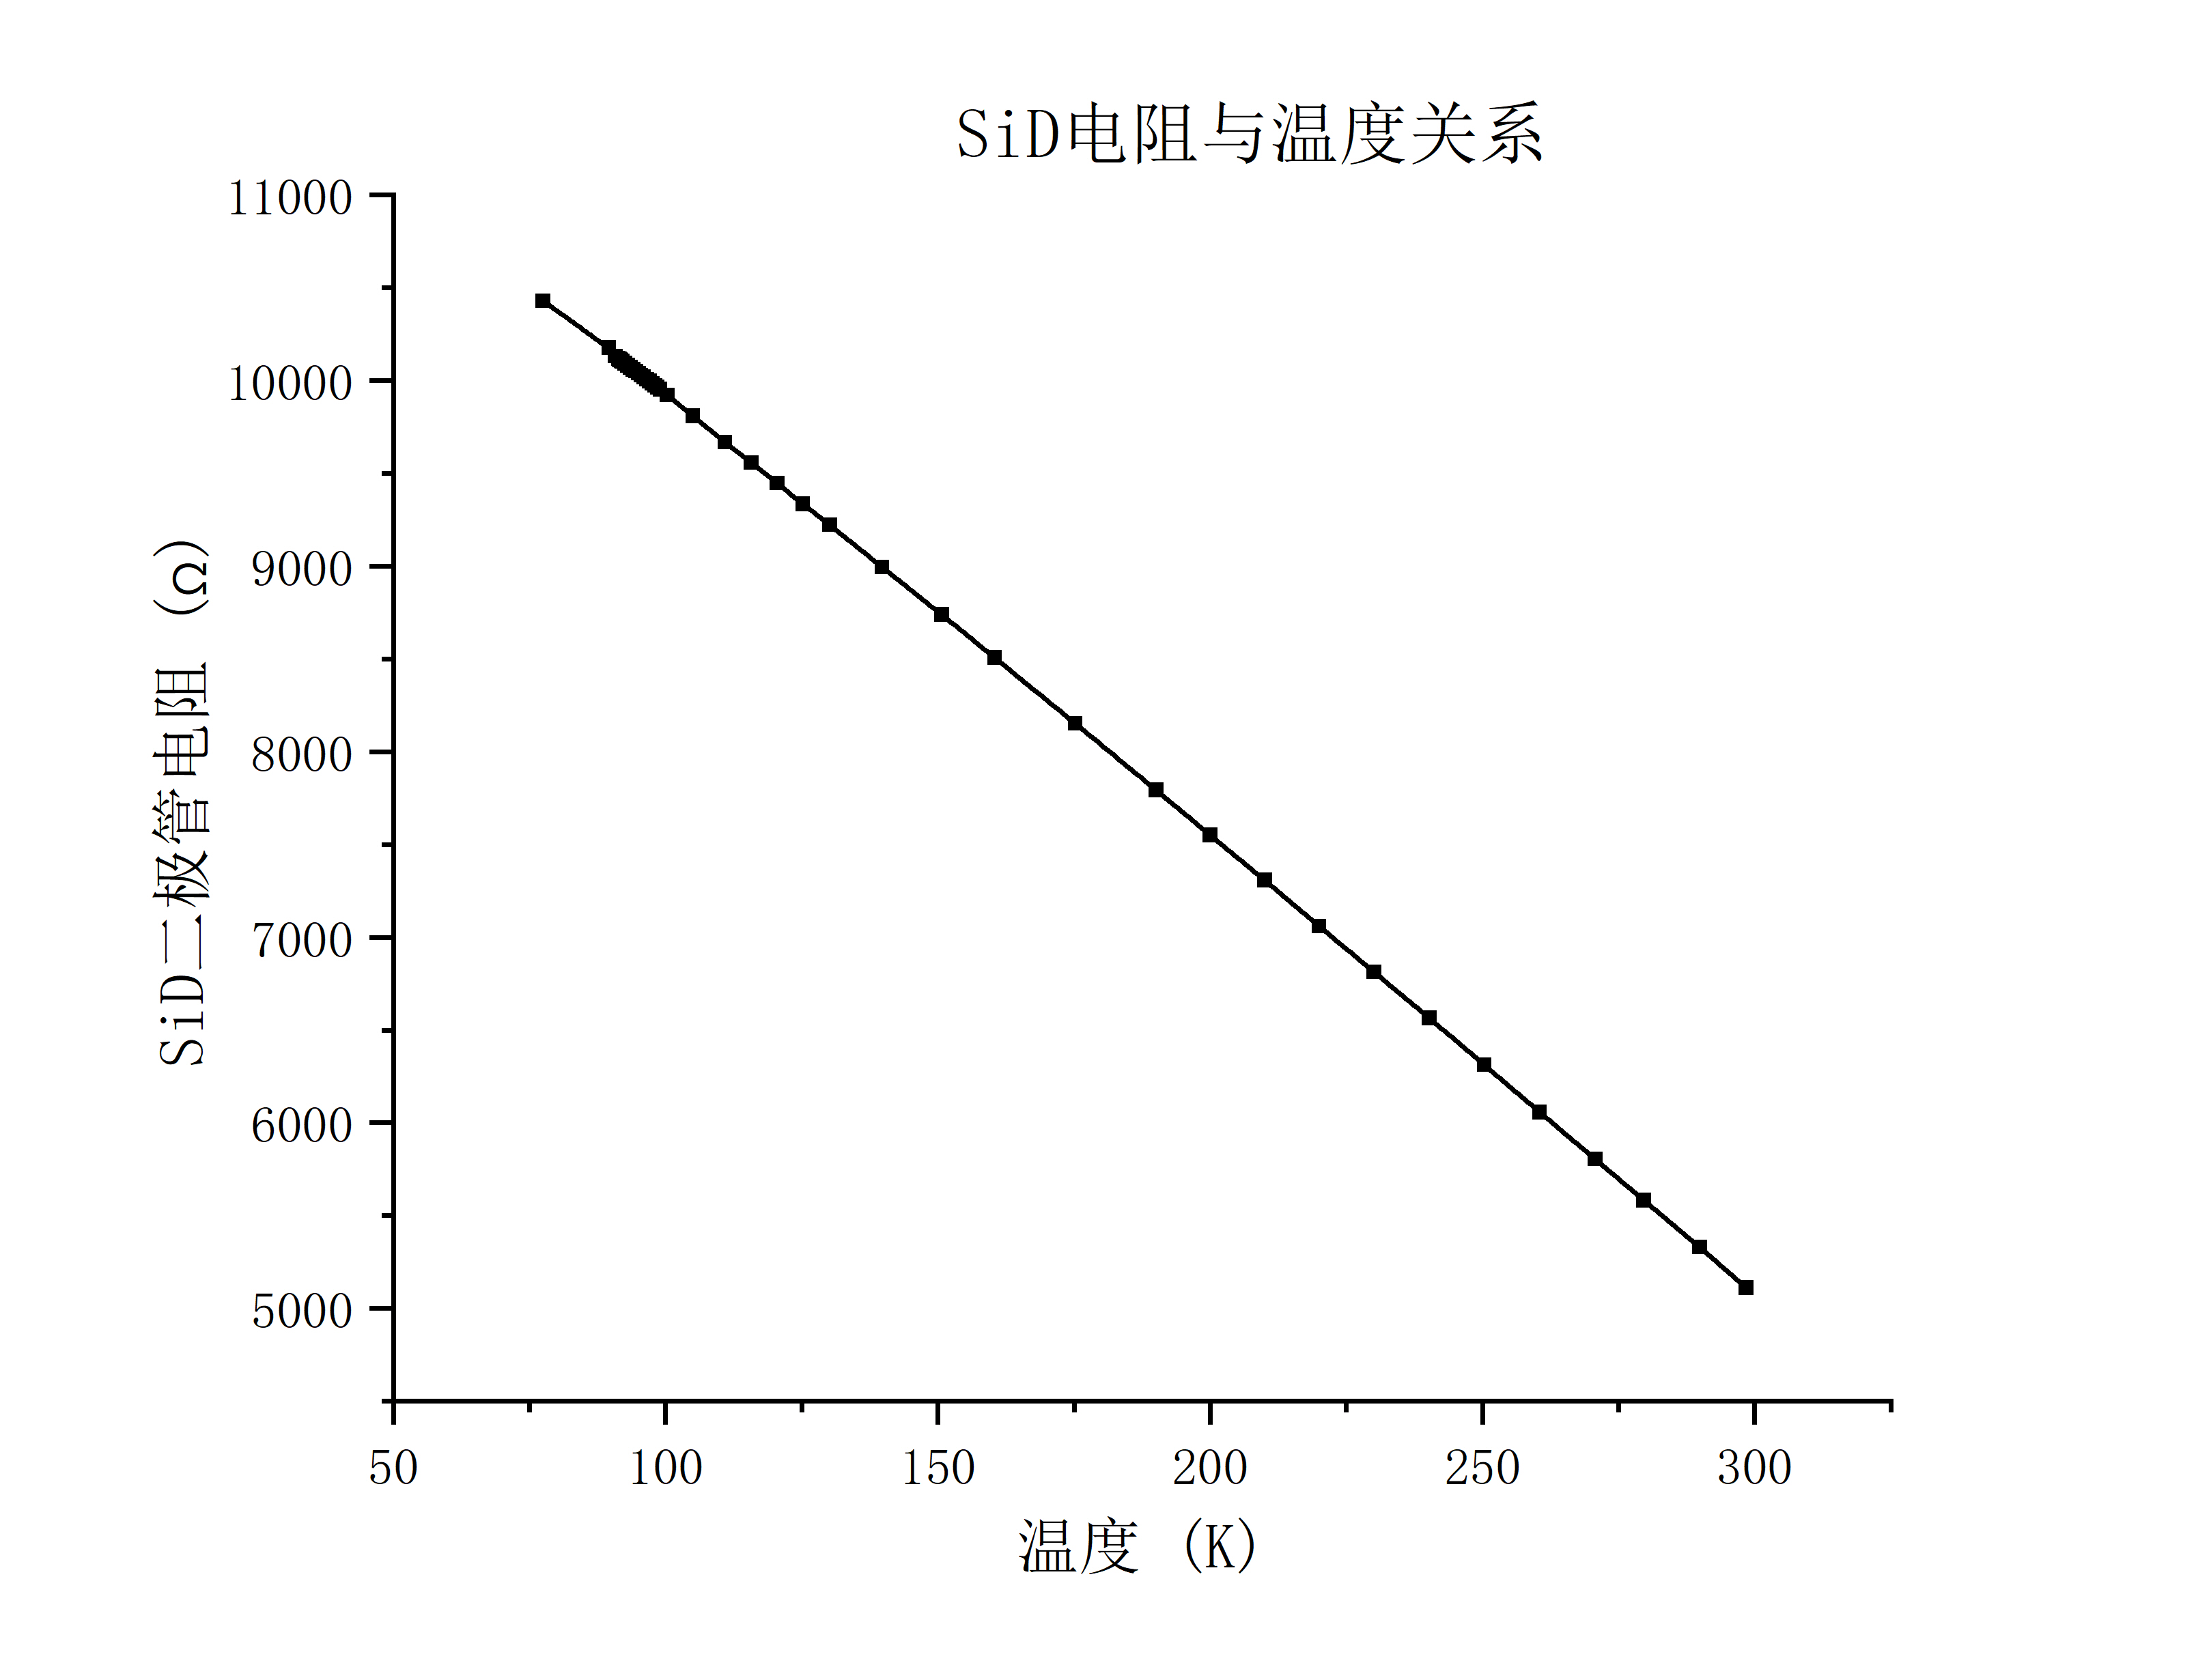
\includegraphics[width=0.8\textwidth]{SiD.jpg}
        \caption{SiD与温度关系}
    \end{figure*}

    \begin{figure*}[htbp]
        \centering
        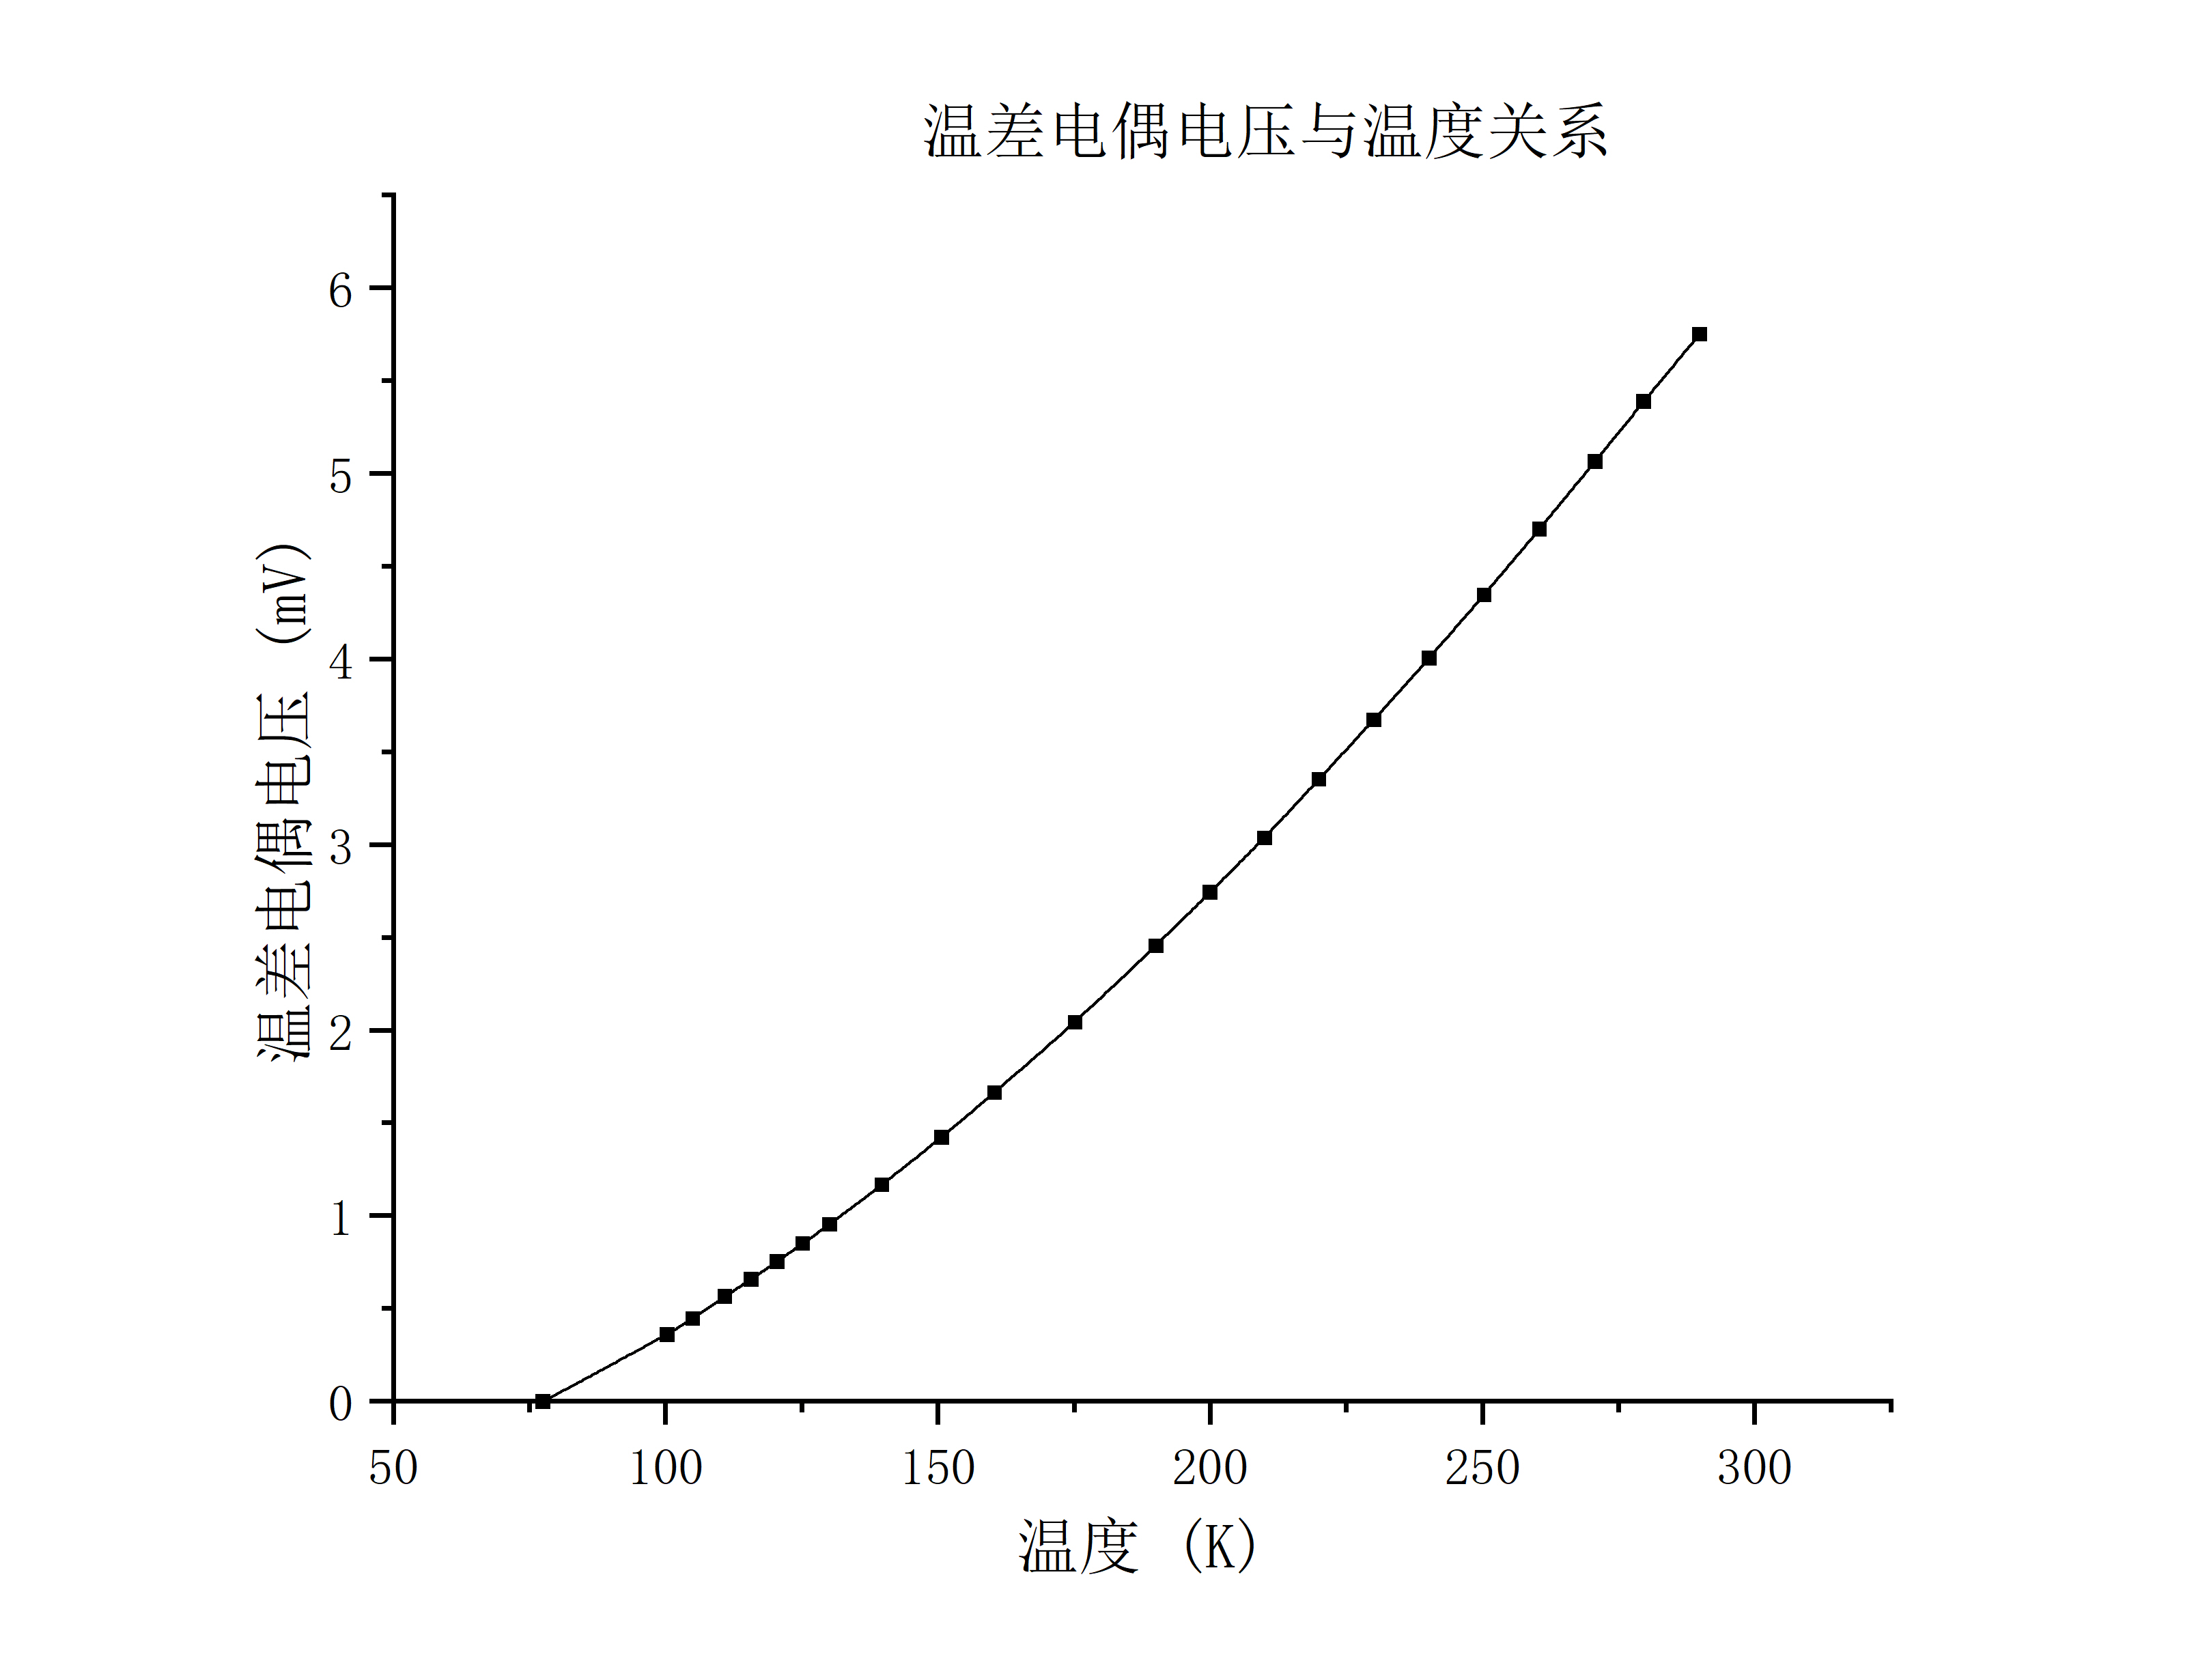
\includegraphics[width=0.8\textwidth]{温差电偶.jpg}
        \caption{温差电偶电压与温度关系}
    \end{figure*}

    根据实验手册给出的铂电阻与温度的关系可以看出,在温度不是非常低的情况下(>13K),铂电阻的阻值与温度之间成线性关系,温度越高,电阻越大;
    而根据实验测得的数据和绘制的曲线可以看出,Si二极管的电阻与温度成反相关,温度越低,电阻越大,且就实验测量的温度范围而言,两者之间也有很好的线性关系,
    如果用最小二乘法对实验中SiD的阻值与温度之间进行线性拟合,相关系数可达到$r=0.99993$,可见线性程度相当高;而温差电偶上的电动势则与温度成正相关,
    即温度越高,电压越大,且随着温度升高,曲线上升得越来越快,即电压的增量随温度升高而增大。

    \subsection{超导样品数据}
    绘制超导样品的阻值随温度的变化曲线,如图3所示。
    
    用最小二乘法对温度在室温到130K之间的数据进行线性拟合,得到直线$l_1$如图4所示,$l_1$同时也显示在图3中,为品红色斜线段。
    li的解析式为$R_1=A T + B$,其中$A=4.9749\times 10^{-5} \Omega/K$,$B=0.00201\Omega$,直线的相关系数为$r=0.9993$。

    样品的电阻曲线在T=110.9K时开始偏离$l_1$,因此$T_{c,onset}=110.9K$。

    $T_{cm}$需要由相变段的直线和$l_2=\frac{1}{2}l_1$确定。$l_2$的解析式为$R_2=\frac{1}{2}(A T + B)$,其中A、B的取值和$R_1$中相同。
    本实验中,相变段的曲线已经非常接近竖直线,实际上有多个温度都会出现同一个温度对应多个不同电阻值的情况。我们最终选取了$T=91.5K$作为相变段直线。
    因此可得两直线交点,即$T_{cm}=91.5K$。

    $T_{c0}$为最终样品电阻刚达到0时对应的温度,反应在实验中是样品上电压刚达到一个接近0并不再变化的电压对应的温度。由于乱真电动势的存在,本实验的最终电压是在-0.002和-0.003之间跳动,
    按下电流方向开关前后电压都在这两个值上跳动。实验中,刚达到这种电压的温度是90.8K。此时样品上的电流为$I=10.0110mA$,比实验开始时略大,不过由于有效数字的限制,并不会反应在电阻值上。
    综合考虑,取$T_{c0}=90.8K$。

    \begin{figure*}[htbp]
        \centering
        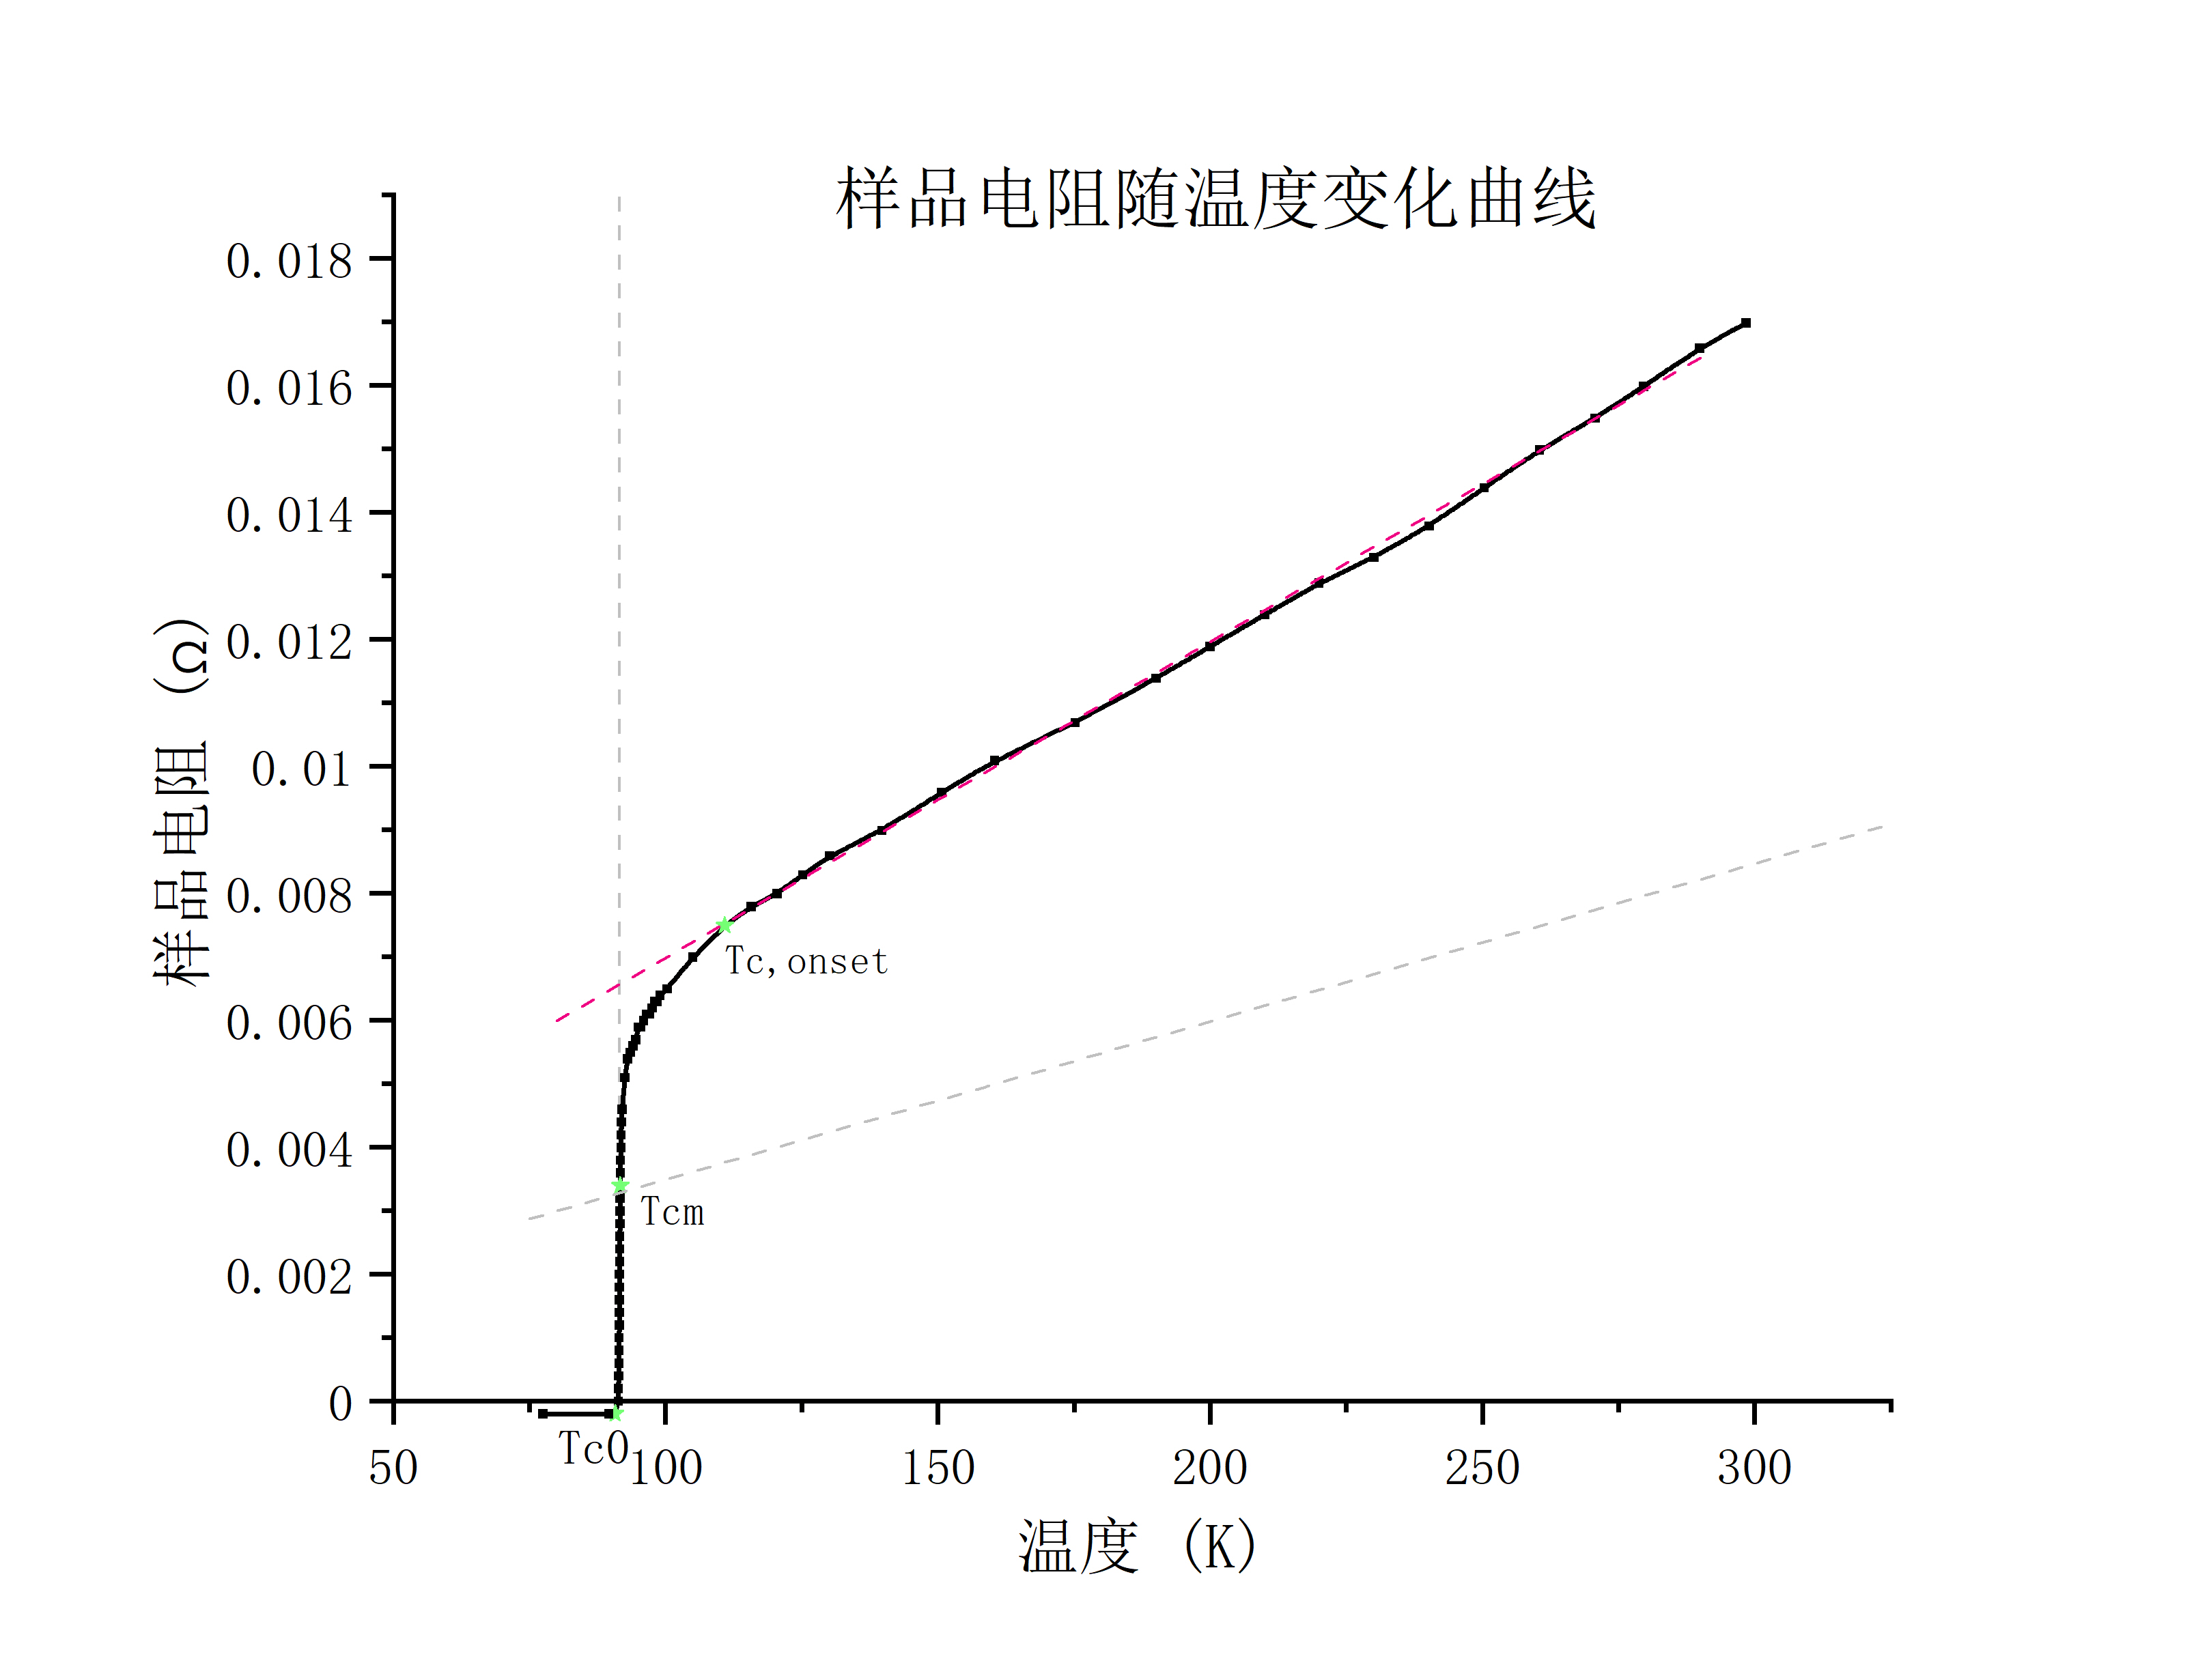
\includegraphics[width=0.8\textwidth]{样品电阻.jpg}
        \caption{超导样品的阻值随温度的变化}
    \end{figure*}

    \begin{figure*}[htbp]
        \centering
        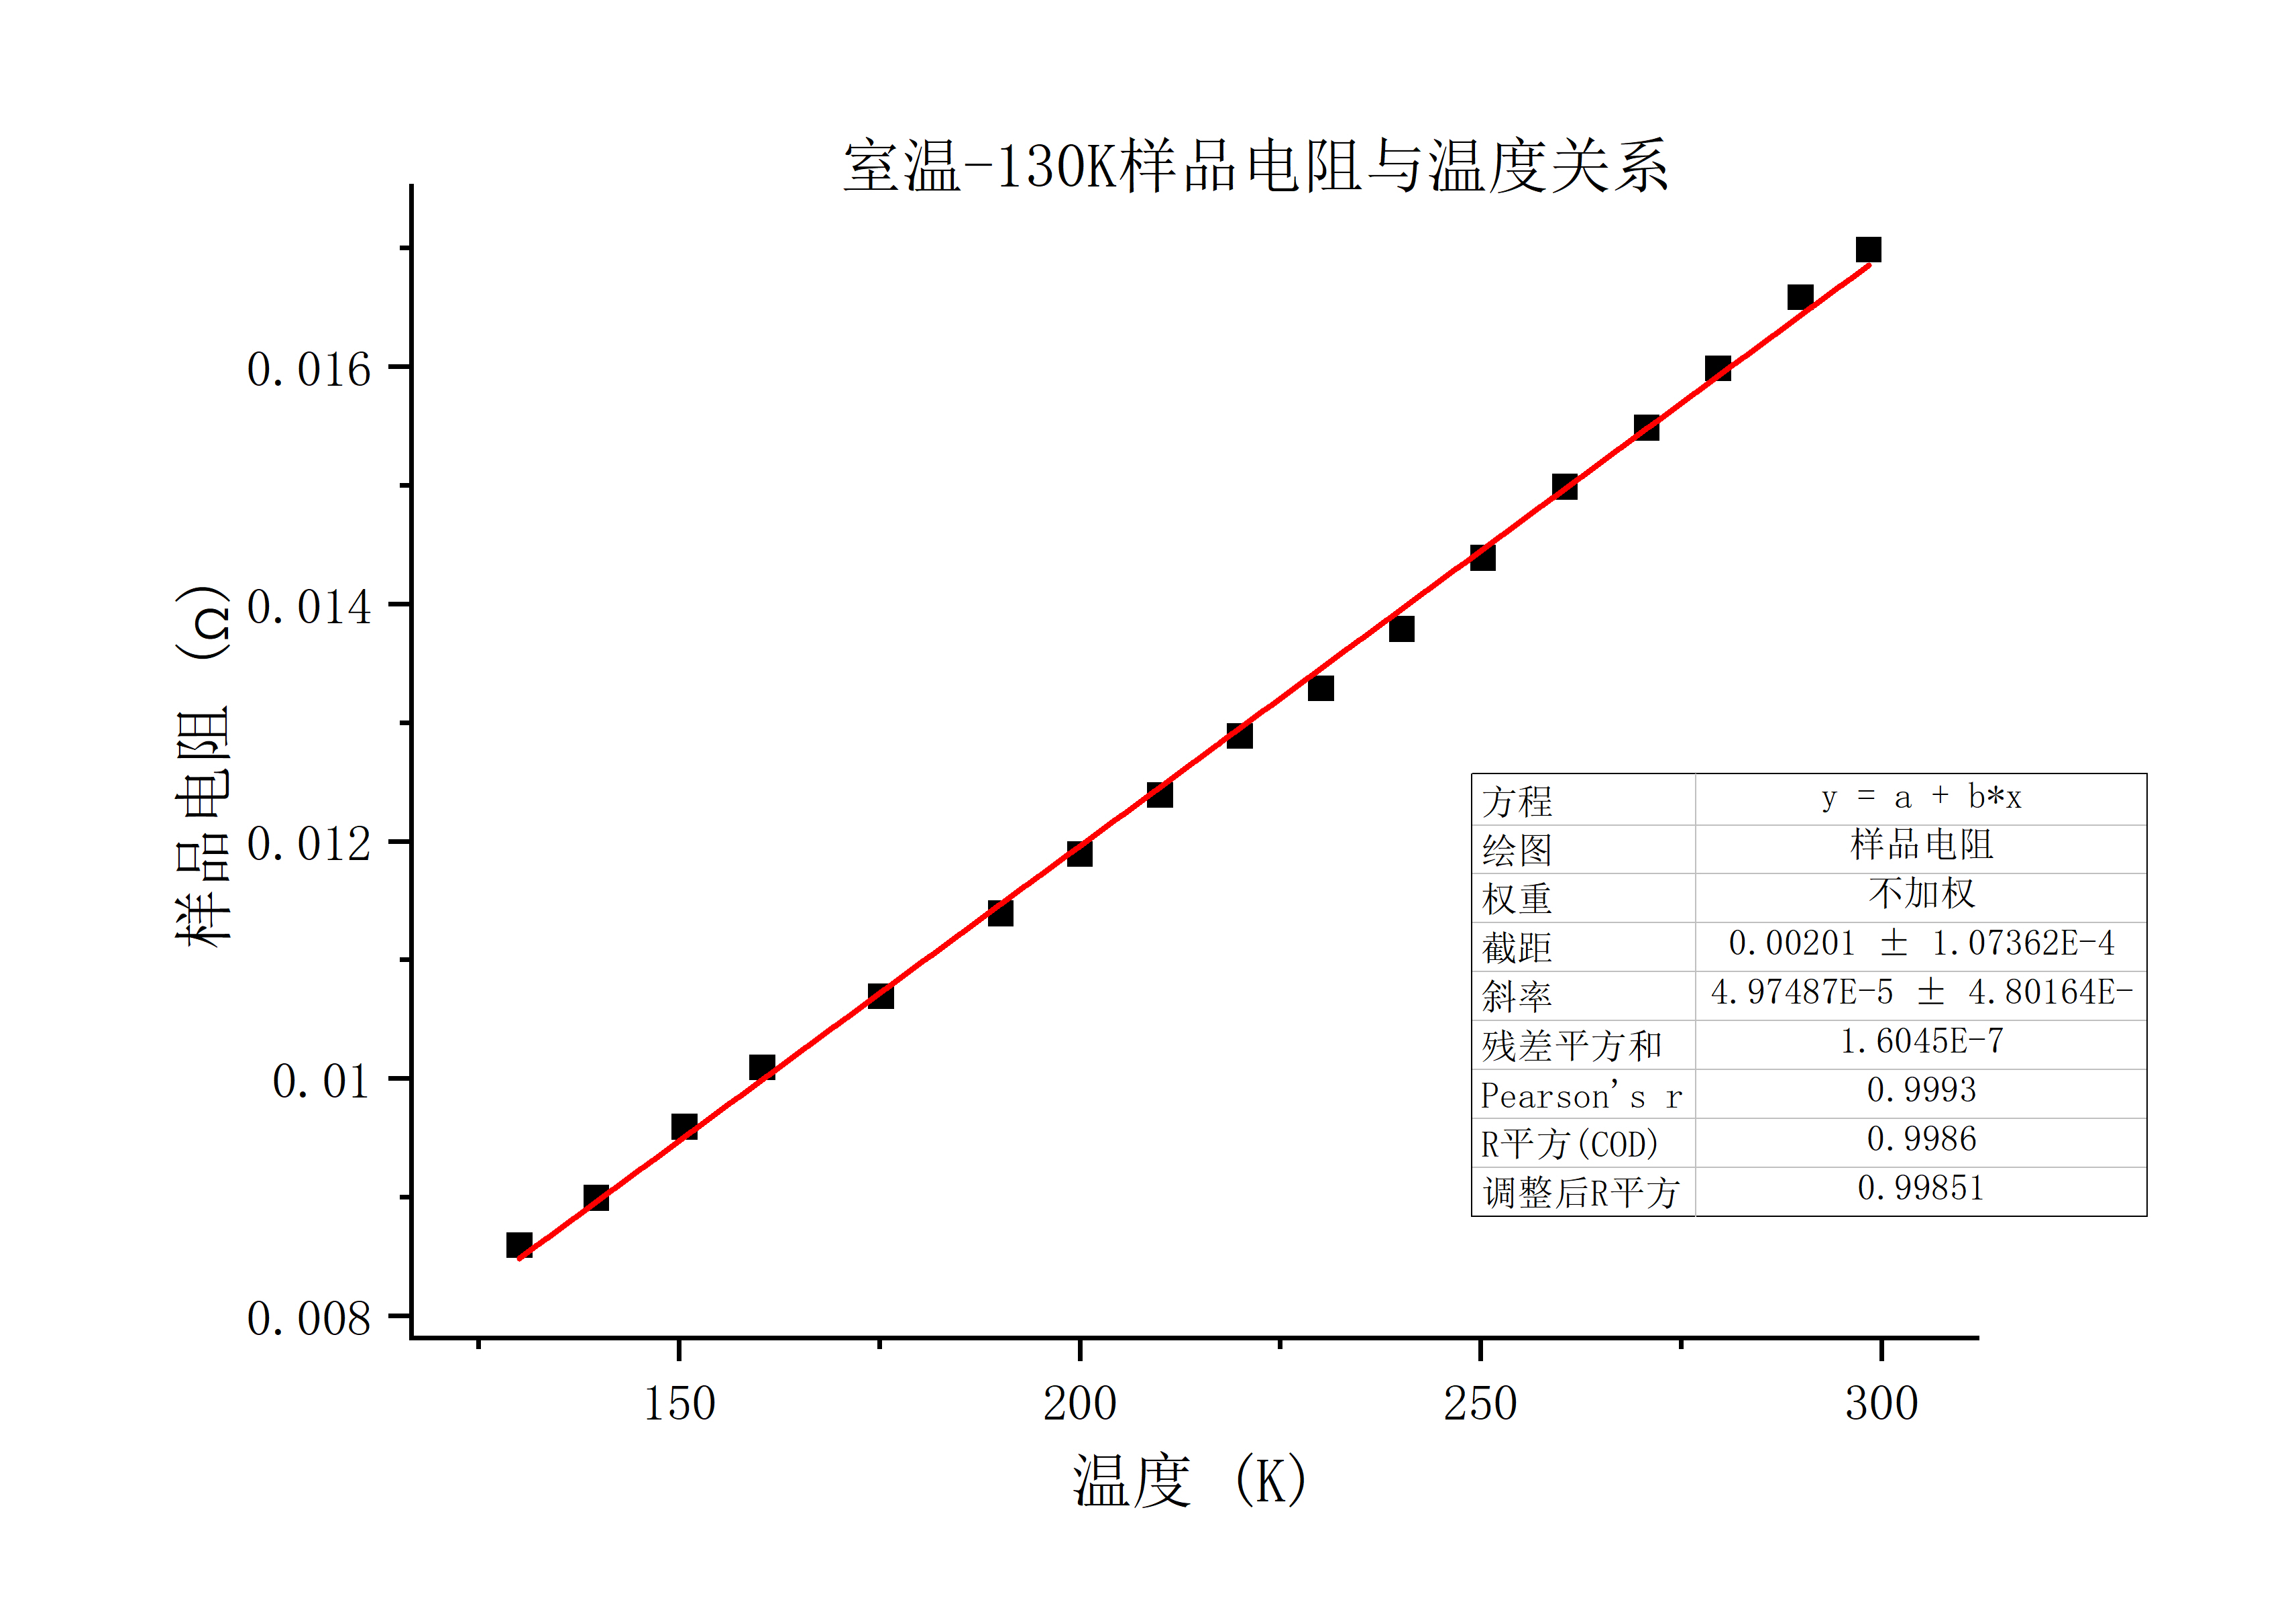
\includegraphics[width=0.8\textwidth]{室温-130K.jpg}
        \caption{最小二乘法拟合室温到130K数据}
    \end{figure*}

    \subsection{液氮沸点检测数据}
    液氮沸点相关的实验数据已经呈现在表1的最后一行。实验测得的液氮沸点为$T=77.4K$,此时SiD上的电压$U_{SiD}=1.0430V$,对应的电阻为$R_{SiD}=1.430\Omega$。
    温差电偶上的电压为$U_{\text{温差电偶}}=-0.001mV$,样品上电压在-0.002和-0.003之间跳动(因受乱真电动势影响),样品上电流为$I=10.0110mA$,样品电阻因此为$R=(-0.0002\sim-0.0003)\Omega$。

    此时再去测量三个测量电路中的电流,Pt电阻测量电路中的电流为$I=1mA$,SiD上的电流为$I=0.1mA$,样品上的电流为$I=10.0110mA$。可以看出,Pt电阻和SiD的测量电路中恒流源的稳定性还是比较好的,样品电压测量电路中恒流源稳定性稍差,
    但对实验结果影响不大。

    \section{分析与讨论}
    实验中样品的$T_{c,onset}$的参考值为92-98K左右,但实际测得的为110.9K,远高于参考值;而$T_{c0}$的参考值为90-92K,实测值为90.8K,与参考值符合得比较好。
    出现这种现象可能是因为样品使用得时间过长,性能下降,已经有点失超了,这会导致$T_{c,onset}$变大而$T_{c0}$基本上不受影响。所以实验中测得的$T_{c,onset}$很大。

\end{document}